% === [ Verification ] =========================================================

\section{Verification}
\label{sec:verification}

% TODO: Add meta-text which mentions verification, performance testing and
% Continuous Integration.

foo

% --- [ Correctness of Implementation ] ----------------------------------------

\subsection{Correctness of Implementation}

foo

\subsubsection{Test Cases}

% TODO: Add
%    - Use the Clang compiler to produce test cases, as it is capable of emitting LLVM IR from C source code. The goal will be to reconstruct the high- level control flow structures (such as for- loops, if-else statements, etc) of the original C code from the LLVM IR.

foo

\begin{figure}[htbp]
	\begin{center}
		\begin{verbatim}
$ go test -v github.com/mewrev/graphs/iso
=== RUN TestCandidates
--- PASS: TestCandidates (0.02s)
=== RUN TestEquationSolveUnique
--- PASS: TestEquationSolveUnique (0.00s)
=== RUN TestEquationIsValid
--- PASS: TestEquationIsValid (0.22s)
=== RUN TestIsomorphism
--- PASS: TestIsomorphism (0.18s)
=== RUN TestSearch
--- PASS: TestSearch (0.20s)
PASS
ok     github.com/mewrev/graphs/iso   0.62s
		\end{verbatim}
		\caption{An extract of the test cases used to verify the subgraph isomorphism search algorithm, as visualized by \texttt{go test}.}
		\label{fig:iso_test_cases}
	\end{center}
\end{figure}

\subsubsection{Code Coverage}

\textbf{NOTE}: \textit{The following section is under construction :)}


The code coverage is a measurement of how much of the code is exercised by the test cases.

% TODO: Add note on how the Go code coverage is calculated.

While developing a lexer for the LLVM IR assembly language the intention was to strive for a 100\% code coverage of any code related to lexing and not related to input output errors (e.g. ``file not found'' errors). As illustrated in figure \ref{fig:lexer_code_coverage}. The rigid testing made it possible to locate and correct a number of faulty assumptions in the lexing logic.

\begin{figure}[htbp]
	\begin{center}
		\begin{verbatim}
$ go test -coverprofile=lexer.out github.com/mewlang/llvm/asm/lexer
$ go tool cover -func=lexer.out
llvm/asm/lexer/lexer.go:36:    ParseFile      80.0%
llvm/asm/lexer/lexer.go:118:   emit           100.0%
llvm/asm/lexer/lexer.go:139:   next           100.0%
llvm/asm/lexer/lexer.go:158:   accept         100.0%
llvm/asm/lexer/state.go:38:    lexToken       100.0%
llvm/asm/lexer/state.go:131:   lexComment     100.0%
…
llvm/asm/lexer/state.go:364:   lexQuote       100.0%
llvm/asm/lexer/state.go:585:   unescape       100.0%
total:                         (statements)   97.5%
		\end{verbatim}
		\caption{A summary of the code coverage for a selection of the LLVM IR lexer functions, as visualized by the \texttt{cover} tool.}
		\label{fig:lexer_code_coverage}
	\end{center}
\end{figure}

The use of code coverage heat maps, which track how often statements are exercised by the test cases, were invaluable when stress testing the subgraph isomorphism search algorithm, and they were able to identify several tricky corner cases. foo figure \ref{fig:iso_heat_map}

\begin{figure}[htbp]
	\begin{center}
		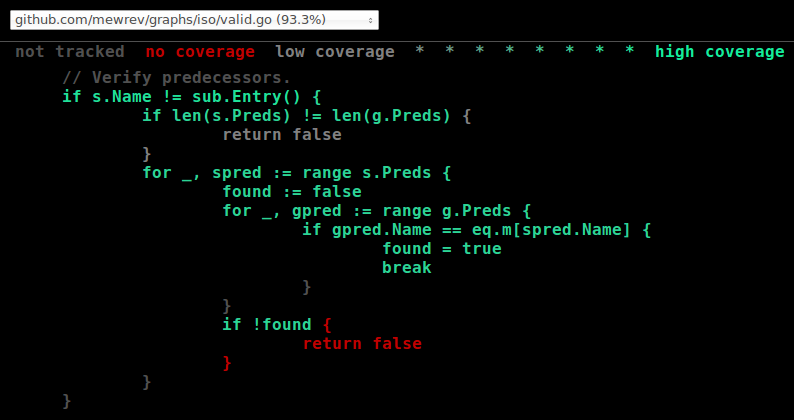
\includegraphics[width=\textwidth]{inc/iso_code_coverage_heat_map.png}
		% TODO: Fix caption text.
		\caption{Extract from the code coverage of the subgraph isomorphism search algorithm, represented as a heat map where red indicates that a statement was never visited and the intensity of green indicates the number of times a statement was visited. where bright green represents a statements that has been visited several times, faint green a statement only visited a few times, and red a statement that has never been visited.}
		\label{fig:iso_heat_map}
	\end{center}
\end{figure}

foo

% --- [ Performance ] ----------------------------------------------------------

\subsection{Performance}

% TODO: Rewrite, cleanup and verify (especially the \theta(...) claims!).

\textbf{NOTE}: \textit{The following paragraph is more of a brain-dump. It will be used as a basis for a future rewrite.}

Profiling was put to good use when optimizing the lexer, the code base of which is rather straight forward. When estimating the runtime complexity of the subgraph isomorphism search algorithm however the use of intuition and algorithm research was far more valuable. For this specific task the generic problem (subgraph isomorphism search of arbitrary input graphs) could be simplified (TODO: use generalized instead of simplified?) to a much easier problem as every node of the graph were known to be connected (TODO: find the succinct term in graph theory to express this concept). Exploiting this property lead to an algorithm that had a runtime complexity of $ \Theta(n*m) $ where $ m $ is known to be small rather than $ \Theta(n^m) $ as is the case for a brute force algorithm and $ \Theta(n^log(m)) $ (TODO: Find the correct runtime complexity of the Hillman iso search algo) as was the case of the Hillman subgraph isomorphism search algorithm which is capable of solving the generic case, improving on the brute force approach by applying heuristics (TODO: is heuristics the right word to use here?) to prune the search space.

In summary, using profiling is great for simple problems. Using algorithm research, runtime complexity theory and intuition is needed for complex problems. Knowledge about specific properties of the problem which may be exploited.

foo

\subsubsection{Benchmarks}

percentage delta.

foo

\texttt{benchcmp}

foo

\subsubsection{Profiling}

% TODO: Add bottle neck example
%    inc/lexer_pprof_before.svg

% TODO:
%    - CPU profiling
%       go test -cpuprofile=a.out
%    - Memory profiling
%       go test -memprofile=a.out

\texttt{go tool pprof}

foo

% --- [ Security Assessment ] --------------------------------------------------

\subsection{Security Assessment}

% TODO: Section moved here from the Design section. Adapt the text to make it fit.

To assess the security of the decompiler pipeline, lets imagine a scenario in which users are given access to the implementation details and source code of the entire system and may provide arbitrary input to any of its components. A potential scenario could involve a web site which provides decompilation as a service and allows its users to interact with the various stages of the decompiler pipeline. The Retargetable Decompiler (see section \ref{sec:retargetable_decompiler}) provides such a service, except it only allows users to interact with the binary analysis stage of the pipeline (see section \ref{sec:binary_analysis}) and its source code is proprietary. The scope of this security assessment will be limited to the various components of the decompiler pipeline and their interaction. In particular security issues related to the operating system, network stack, web server and web site (e.g. SQL-injection and XSS vulnerabilities) of the decompilation service are intentionally excluded from the scope of the security assessment.

The objective of an attacker may be to escalate their privileges in a system by exploiting it to execute actions not intended by design. Since the security of any system is only as strong as its weakest link, it is critical to identify and isolate likely targets for attacks. Projects which consist of or depend on large C or C++ code bases may exhibit memory safety issues, such as buffer overflows or use-after-free vulnerabilities. These issues are considered low-hanging fruit for attackers and have a long history of successful exploitation \cite{for_fun_and_profit}. Several modern programming languages (including Go) provide memory safety guarantees and may solve these issues by inserting bounds-checking for array accesses and using garbage collection for memory management. Code written in memory safe languages may still contain other security vulnerabilities caused by logic errors or insufficient validation, sanitation and parametrization of input (e.g. command injection and directory traversal vulnerabilities).

The number of lines of code in a project may give an indication to the project's complexity and to some extent its potential attack surface. As summarized in table \ref{tbl:loc_summary} every component of the decompiler pipeline except \texttt{iso} depends on LLVM. The LLVM code base contains approximately 800~000 lines of C++ source code, and even if only a portion of the code will be linked into the executables it is an interesting target for attacks. One thing to keep in mind is that there are several high-end users of the LLVM project (such as Apple, Intel, NVIDIA and Sony \cite{llvm_users}) and it has a well established code reviewing process. Some of the LLVM developers are also very well educated in common security vulnerabilities and have developed the Clang Static Analyzer, which is a static source code analysis tool that locates bugs (such as buffer overflows and use-after-free issues) in C and C++ programs \cite{clang_analyzer}. The LLVM project may contain several security issues due to its size, but they are most likely difficult to discover since the low-hanging fruit have been caught already by the Clang Static Analyzer. Similarly, Google Protocol Buffers are used extensively by several companies and organizations and the likelyhood of discovering a simple security vulnerability in its code base is low.

\begin{table}[htbp]
	\begin{center}
		\begin{tabular}{|l|l|l|l|}
			\hline
			\textbf{Project} & \textbf{Language} & \textbf{Lines} & \textbf{Dependencies} \\
			\hline
			\multicolumn{4}{|l|}{\hspace{4ex} \textit{Front-end}} \\
			\hline
			Dagger & C++ & 2~000 & LLVM \\
			Fracture & C++ & 20~000 & LLVM \\
			MC-Semantics & C++ & 25~000 & LLVM and Google Protocol Buffers \\
			\hline
			\multicolumn{4}{|l|}{\hspace{4ex} \textit{Middle-end}} \\
			\hline
			ll2dot & Go & 500 & LLVM and dot \\
			iso & Go & 2~000 & dot \\
			\hline
			\multicolumn{4}{|l|}{\hspace{4ex} \textit{Back-end}} \\
			\hline
			ll2go & Go & 1~500 & LLVM, llvm (Go), iso and dot \\
			\hline
			\multicolumn{4}{|l|}{\hspace{4ex} \textit{Dependencies}} \\
			\hline
			LLVM & C++ & 800~000 & - \\
			Google Protocol Buffers & C++ & 125~000 & - \\
			llvm (Go) & Go & 5~000 & - \\
			dot & Go & 7~000 & - \\
			\hline
		\end{tabular}
	\end{center}
	\caption{A rough summary of each project specifying their programming language, number of lines of code and dependencies.}
	\label{tbl:loc_summary}
\end{table}

There are still three potential targets which may contain memory related vulnerabilities, namely the front-end projects which translate binary executables, object code and shared libraries to LLVM IR.

foo

% easy to make mistakes in the parsing logic. Trust header fields without verifying.

% TODO: Mention the unnamed hack (gain access to the names of anonymous basic blocks).
%    - Unable to trust the integrity of the output of local files are tampered with. Trusting trust.

% TODO: Security through obscurity
% TODO: Defence in depth
%    - Use several layers of security such that one may fail without disrupting the integrity of the entire system (e.g. jail [chroot on steroids])
% TODO: Memory Safety
%    - Mitigated using security through obscurity (e.g. ASLR, ) and true security (e.g. W^X).

% --- [ Continuous Integration ] -----------------------------------------------

\subsection{Continuous Integration}

% TODO: Move CI from Verification to Methodology?

The Continuous Integration (CI) practise originated from the Extreme Programming methodology \cite{xp} but has reached a much broader audience in recent years. Today most large scale software projects rely on CI server farms which continuously compile and test new versions of the source code.

This project makes use of Travis CI, which is tightly integrated with GitHub, to run a series of automated tests for each commit to the source code repository. The tests are varied and range from identifying source code formatting and coding style issues to monitoring the build status and test coverage. A future ambition is to run benchmarks for each commit to quickly identify performance regressions.

\subsubsection{Source Code Formatting}

Instead of relying on a formatting style guide the Go project enforces a single formatting style using \texttt{gofmt} (a tool similar to \texttt{indent}) which automatically formats Go source code. The adoption of this tool is widespread within the Go community as indicated by a survey conducted back in 2013. The survey found that 70\% of the publicly available Go packages were formatted according to the rules of \texttt{gofmt} \cite{gofmt_70percent}, a figure which is likely to have increased since then.

Using a single formatting style for all Go source code may at first seem like a small deal, but the advantages are vast. It becomes easier to write code as one may focus on the problem at hand rather than minor formatting issues. Similarly it becomes easier to read code when it is formatted in a familiar and uniform manner. We may focus our entire attention at understanding the semantics of the code without being distracted by inconsistent or unfamiliar formatting. And perhaps most importantly, it prevents useless discussions about which formatting style is the right one.

Several text editors supports adding pre-save hooks which executes a command to pre-process the text before saving it. This mechanism may be used with the \texttt{gofmt} tool to automatically enforce its formatting style each time a source file is saved. One of the CI tests catches and reports incorrectly formatted source code, should a programmer forget to install such a hook.

\subsubsection{Coding Style}

% There exists linting software for several programming languages which detect and report issues related to coding style.

% The established conventions

% There exists several official sources which describe the coding conventions

% Effective in the sense that

% Learning the syntax of a programming langauge and its key features is not enough to ensure

% TODO: Add paragraph refering to Effective Go.
% \cite{effective_go}

% TODO: cyclocomplexity...?

% To write idiomatic code in any programming language requires at least a resonable understanding of underlying design decisions which drove the development of the language.

% a understanding of its is required of the

% Learning to program effectively in a new language requires much more than simply learning the syntax of the language and its key features. A reasonable understanding of the underlying design decisions behind the language,

% When learning a new programming language it is important to understand its ideoms and the established conventions.

% The conventions

% Coding conventions

foo

\texttt{golint}

% * Key word, conventions.
%
% := type inference.
% naming conventions
% documentation comments
% error messages

\cite{golint}

foo

\subsubsection{Code Correctness}

\texttt{go vet}

foo

\subsubsection{Build Status}

\texttt{go get}

foo

\subsubsection{Test Cases}

\texttt{go test}

foo

\subsubsection{Code Coverage}

\texttt{go test -cover}

foo
